\documentclass[journal]{IEEEtran}
%
% If IEEEtran.cls has not been installed into the LaTeX system files,
% manually specify the path to it like:
% \documentclass[journal]{../sty/IEEEtran}

\makeatletter
\def\markboth#1#2{\def\leftmark{\@IEEEcompsoconly{\sffamily}\MakeUppercase{\protect#1}}%
\def\rightmark{\@IEEEcompsoconly{\sffamily}\MakeUppercase{\protect#2}}}
\makeatother

\usepackage[latin1]{inputenc}
\usepackage[T1]{fontenc}
\usepackage{cite}
\usepackage{graphicx}
\usepackage{url}
\usepackage[norsk,english]{babel}
\usepackage{amsmath}
\usepackage{verbatim}
\usepackage{varioref}
\usepackage{color}
\usepackage{listings}
\usepackage{epsfig, times}

%\usepackage[cmex10]{amsmath}
%\usepackage{algorithmic}
%\usepackage{array}
%\usepackage{mdwmath}
%\usepackage{mdwtab}
%\usepackage[tight,footnotesize]{subfigure}
%\usepackage[caption=false]{caption}
%\usepackage[font=footnotesize]{subfig}
%\usepackage[caption=false,font=footnotesize]{subfig}
%\usepackage{fixltx2e}
%\usepackage{stfloats}

% correct bad hyphenation here
\hyphenation{net-works}


\begin{document}

\title{Implementation of CacheCast\\ in the ns-3 network simulator}

\author{Bekzhan~Kassymbekov,~
        Dag~Henning~Liodden~S�rb�,~
        Kanat~Sarsekeyev,~
        and~Rizwan~Ali~Ahmed}% <-this % stops a space

% \thanks{J. Doe and J. Doe are with Anonymous University.}% <-this % stops a space
% \thanks{Manuscript received April 19, 2005; revised January 11, 2007.}}

% The paper headers
% \markboth{Journal of \LaTeX\ Class Files,~Vol.~6, No.~1, January~2007}%
% {Shell \MakeLowercase{\textit{et al.}}: Bare Demo of IEEEtran.cls for Journals}


%%---------------------------------------------------------------------------%%
% make the title area
\maketitle


\begin{abstract}
This paper will introduce and explain the implementation of the CacheCast system in the ns-3 
network simulator. Several aspects of the implementation and views on it will be 
presented. We will let the user know how it should be used in simulations and 
for the developer we present the details of the implementation. Tests and 
evaluations has been performed to prove that the implementation follows the 
design of the CacheCast mechanism. The outcome of this work is an 
independent ns-3 module called \emph{cachecast} which contains all functionality 
to create ns-3 simulations with the CacheCast technique.
\end{abstract}


% \begin{IEEEkeywords}
% IEEEtran, journal, \LaTeX, paper, template.
% \end{IEEEkeywords}


\section{Introduction}
\IEEEPARstart{T}{he} CacheCast system is a new technique which removes redundant 
payload on Internet links. The system is currently implemented in the Linux 
operating system, the Click modular router and partially in the ns-2 network 
simulator. In order to test new techniques and protocols destined for the 
Internet, network simulators are often used. A new network simulator called ns-3 has been developed which
focuses on more accurate modeling of the functionality of a modern network. The 
goal of this work is to implement the CacheCast system in the ns-3 network 
simulator.

The implementation will consist of a ns-3 module which contains the data 
structures and the algorithms for the CacheCast packet handling. The module will 
also contain example scripts and demos to make it easy the see how the module is 
used in ns-3 network simulations.

This document is structured in the following way. In section \ref{s1} we give a brief 
description of the CacheCast system and we follow up which an introduction to 
the ns-3 network simulator in section \ref{s2}. Then we present the API of the 
implementation in section \ref{api}. In section \ref{s4} we dive into the 
details of the implementation and perform an implementation evaluation in 
section \ref{s5}. We give our conclusions in section \ref{s6}. We start now by 
getting to know the CacheCast system design.


\section{The CacheCast system\label{s1}}

\begin{figure}[!t]
\centering
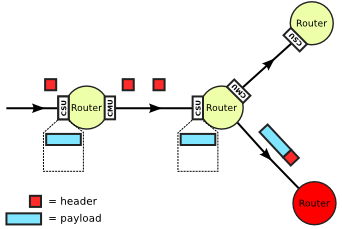
\includegraphics[width=3.5in]{cachecast}
\caption{The packet modification in the CacheCast system}
\label{fig_cachecast}
\end{figure}

CacheCast\cite{srebrny} is a new technique of removing redundant data packets on 
a link. The purpose of CacheCast is to remove as much as possible of the 
overhead when using many unicast connections for the same data over the same 
link. In short, CacheCast only sends the packet payload once over a link 
together with the destination addresses, and then the responsibility lies on the 
router on the link exit to forward the payload to each client. With this 
redundancy removal, CacheCast achieves close to multicast performance when the 
numbers of receivers grow large, without introducing any new protocols into the 
Internet. An overview of the CacheCast packet modification can be seen in figure 
\ref{fig_cachecast}.

As the name implies, CacheCast uses caching to remove the redundant data packets 
from a link. Three main components are needed to make CacheCast work; support 
for CacheCast on the server, a component on the link entry called \emph{Cache 
Management Unit (CMU)} and a component on the link exit called \emph{Cache Store 
Unit (CSU)}. It is important to notice that these components can be divided into 
two groups; server support and network support. These two groups work 
independently of each other. Hence, there is no communication between the server and the 
components in the network. Each CacheCast packet contains a CacheCast header. It 
contains three fields; payload size (\emph{P\_SIZE}), payload id (\emph{P\_ID}) 
and cache index (\emph{INDEX}). The details of these fields will be explained in 
the following sections.

\subsection{Server support}
The use of CacheCast demands that the server is aware of CacheCast support 
in the network, thus a server component is needed. Clients connected to the 
server requesting the same content is served via the CacheCast component. To be 
able to take advantage of CacheCast, data should be sent to many clients at the 
same time. This batching of clients is done by applications using the CacheCast 
support.

The responsibility of the server support is therefore to handle this client 
batching. Currently this handling is done through a system call (\textsf{msend()}) 
implemented in the Linux operating system. The input to this system call is a 
set of connections to clients and the data to be sent. The system call will then 
add the CacheCast header to each packet and mark the packets as CacheCast 
packets. This is done to let the other CacheCast components separate CacheCast 
packets from regular packets.

At last the server sends the packets onto the link in a tight sequential order.  
However, only the first packet contains the payload whereas the other packets are 
truncated. Because of this removal of redundant payload the CacheCast packets 
follow a certain pattern. The first packet contains a header and the data, 
whereas the rest of the packets only contain the headers. This structure is 
called a packet train.

\subsection{Network support}
The network support is implemented on a per link basis and consist of two 
components; the CMU located at the entry of a link, and the CSU located at the exit of 
that same link. This way CacheCast support need not be deployed in the whole 
network. It can be deployed incrementally from the server.

Let us now see how this network support is realised through the CMU and the CSU.
 
\subsubsection{CMU\label{cmu}}
The CMU's responsibility is to remove the redundant payload and manage 
the cache in the CSU. For each payload transfered over the link a unique 
payload ID (P\_ID) is given the payload which identifies, together with 
the source address, the payload uniquely in the Internet. If the CMU 
receives a new CacheCast packet with a P\_ID currently in the cache it 
removes the payload from the packet, adds a CacheCast header and sends the 
truncated packet onto to link. The index field in the CacheCast header identifies 
the payload in the cache in the CSU. If the CMU receives a 
CacheCast packet not currently in the cache it assigns a new P\_ID to the 
payload and inserts this ID into a table. The index of this table entry 
corresponds to the slot in the cache in the CSU where the payload will be 
stored. The CMU then adds the CacheCast header to the packet and sends 
the whole packet onto the link.

\subsubsection{CSU\label{csu}}
The CSU is the component containing the actual cache. The data in the 
first packet of the packet train is stored in a slot in this cache specified by 
the CMU. The job of the CSU is to attach the correct payload to 
the packets containing only headers. The router will process each packet as 
normal IP packets.


\section{The ns-3 network simulator\label{s2}}
The ns-3 simulator\cite{ns-3} is a discrete-event network simulator, in which the simulation core and models are implemented in C++. ns-3 is
built as a library which may be statically or dynamically linked to a C++ main program that defines the simulation
topology and starts the simulator. ns-3 also exports nearly all of its API to Python, allowing Python programs to import
an �ns3� module in much the same way as the ns-3 library is linked by executables in C++.

It is an open-source project, intended for educational and 
scientific use. Main purpose for usage of this tool is to simulate  different routing protocols, scenarios that accure in different
network. These scenarios and designs of network are implemented by user. ns-2 is a version prior to ns-3, which is a new simulator 
that does not support the ns-2 APIs. ns-3 supports popular network protocols used nowadays. Some models from ns-2 have already been ported 
from ns-2 to ns-3, and some has not yet been implemented in ns-3. 
Version of ns-3 we are using during  our implementation and simulation is ns-3.13. 

\subsection*{Abstractions}
Implementation in ns-3 is based on abstraction, so it can be simplified. 
These abstraction have differences from the network as we know in reality. 
Before we start explaining our implementation of CacheCast in ns-3, it is 
important to understand abstractions and terms that are used in ns-3.

\subsubsection{Node}
In ns-3 devices like host and end-user are represented as abstractions of 
nodes by the class \texttt{Node}. This class provides management of how these 
devices will be represented in simulations. 

\subsubsection{Application}
Application is abstractions of user programs that are suppose to produce activity 
on nodes to be simulated. This is represented by the class \texttt{Application}, 
which provides methods for managing the representations of applications in simulations.

\subsubsection{Channel}
In ns-3, each Node are connected by a connection that are represented by a communication 
channel. This abstraction is represented by class \texttt{Channel}, which provides methods 
for managing communication subnetwork objects and connecting nodes to them.

\subsubsection{NetDevice}
Net device abstraction covers both the software driver and the simulated hardware. 
A net device is  more or less "installed" in a Node in order to enable the Node to communicate 
with other Nodes in the simulation via Channels. Node may be connected to more than one 
Channel via multiple NetDevices. This abstraction is represented by class \texttt{NetDevice} 
which provides management of connections to Node and Channel.

\subsubsection{Topology Helpers}
In a simulated network, connections between Nodes, NetDevices and Channels needs to be 
arranged. NetDevices needs to be attached on Nodes, Node protocol-stack needs to be configured and a 
communication channels need to be defined between NetDevices and so on. Topology helpers are used 
to arrange these attachments as easy as possible on a large scale.

\section{Application programming interface (API)\label{api}} % HOW TO USE IT
We have now talked about the general design of CacheCast and about the details 
of the ns-3 network simulator. In this section we will explain how the CacheCast 
system is used by script authors. bla bla ...


\subsection{Services provided to applications}
Since end-to-end cachecast connections are handled by different sockets, the send procedure requires 
a sequence of send-requests (corresponding to each socket) to transmit packets to all client. A 
multiple-send-request from application layer requires a container of sockets, so the application can 
send packets through / to all sockets in the container. 

Since a such socket container is not supported by transport layer and nor a part of a application-layer, 
we chose to implement a CacheCast Application Programming Interface in the class \texttt{CacheCast}. 
This interface will not only support the socket container, but also systemcall \texttt{Msend()} 
would be provided to the application. This is much more practical than having a static systemcall 
called by the application.

The socket container itself is implemented as a vector of sockets (\texttt{m\_sockets}), which contains 
sockets added by application. In addition to vector \texttt{m\_sockets} we chose to have another 
vector \texttt{m\_failed} to provide the application the knowledge of sockets that failed during the 
msend procedure.

\begin{footnotesize} 
\begin{lstlisting}[language=C,caption = Services provided to application, 
frame=tb, label=services]
void AddSocket(Ptr<Socket> socket);
void RemoveSocket(Ptr<Socket> socket);
    
void Merge(CacheCast cc);
   
Iterator Begin (void) const;
Iterator End (void) const;
 
Iterator BeginFailedSockets (void) const;
Iterator EndFailedSockets (void) const;

bool Msend(Ptr<Packet> packet);
\end{lstlisting}
\end{footnotesize}
In order to maintain the container of sockets, some facilities are provided to applications. 
It is necessary for the application to add or remove sockets in the container. And the possibility 
to merge two or more socket containers might also become handy. It is described in Listing \ref{services}.
 
%Todo moooore
\subsection{Usage of CacheCast API}

In CacheCache, applications stands for creating and binding sockets and CacheCast API
is responsible for maintaining these sockets. When a socket is binded, it is added in the socket 
container simply by using function AddSocket. 

Packet is sent to all socket in the socket container by using function Msend.  
There is no possibility for applications to have a complete overview of which one of socket did 
failed until the Msend function is completed. We have implemented this function 
to return a bool depending on if packet was delivered succesful to all sockets in the container.
If a socket fails, Msend places that socket in a vector for failed sockets and returns false.
The application would then know there is a socket that failed during sending
procedure. An iterator is provided to the application, so it can iterate through the vector 
containing failed sockets. And it is entirely up to the application how failed socket should be treated.
Implementation of Msend is listed later in this document. 

\begin{footnotesize}
\begin{lstlisting}[language=C, caption = Example of usage of CacheCast API, 
frame=tb]
// assuming socket1 and socket2 is set up and connected
CacheCast cc;
cc.AddSocket (socket1);
cc.AddSocket (socket2);

Ptr<Packet> packet = Create<Packet> (1400);

if(!cc.Msend(packet)){
  CacheCast::Iterator vItr = cc.BeginFailedSockets();
  while ( vItr != cc.EndFailedSockets() )
  {
    cc.RemoveSocket( (*vItr) );
    vItr++;
  }    
}
\end{lstlisting}
\end{footnotesize}

\subsection{Helpers}
Helpers are used to setup the Server Unit / CMU and CSU on nodes before channel between these units 
are defined. In both helpers, Install function takes pointer for two nodes as arguments. The only 
difference between these two helpers is that CacheCastServerHelper is intended to be used to define 
characteristics of connections between Serverunit and CSU and CacheCastHelper is used to define 
CMU and CSU. While defining the server node , CacheCastPid is aggregated
 to the object, so it has abillity to wrap around payload id.  

First, CacheCastNetDevices are created for each of these nodes.

%Todo Mer info

Server unit, CMU or CSU are then added to these devices based on type of node that are being 
installed. These devices are then attached to CacheCastChannel before they are added into a 
container of NetDevices.    


\section{General implementation details\label{s4}} % HOW IT WORKS
In the previous section we looked at the implementation of CacheCast in ns-3 
from the user perspective. In the following sections we will dig deeper into the 
implementation details and look at the implementation from a developer 
perspective. In this section we explain how the CacheCast packets traverse the nodes and 
the channels in order to get a general overview of how the implementation works, 
and we look at common data structures used throughout the implementation. In the 
next two section we elaborate on the specific implementation details for the 
server support and the network support.

\subsection{General overview}
The implementation of CacheCast in ns-3 (as in the general design of CacheCast) 
consists of three main parts; server support, CMU and CSU. As explained in the 
previous section, to support CacheCast, packets are sent with the 
CacheCast::Msend() function in the ns-3 applications on the server node. Then 
the packets traverse the network layers and is intercepted by the CacheCastNetDevice. In 
this CacheCastNetDevice a CacheCastServerUnit is installed which adds a 
CacheCastHeader to the packets and truncates packets with redundant payload. The 
packets then traverse the channel and is received by a CacheCastNetDevice 
on the other end. In this CacheCastNetDevice a CacheStoreUnit is 
installed which adds payload to the truncated packets and remove the 
CacheCastHeader. The packets are then handled as normal IP packets in the node. 
If the packet is destined for another node, it is again intercepted by a 
CacheCastNetDevice in which a CacheManagementUnit is installed. This unit adds 
the CacheCastHeader to the packet and truncates packets with redundant payload. 
The packets then traverse another channel and is received by another
CacheCastNetDevice with a CacheStoreUnit installed. This process is continued 
for each node supporting CacheCast on the packet's path to its destination. An 
graphical overview of this structure can be seen in figure \ref{fig_overview}.

\begin{figure}[!t]
\centering
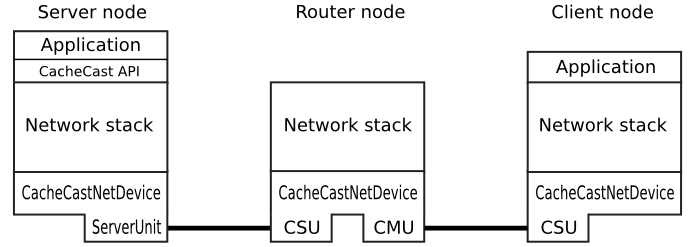
\includegraphics[width=3.5in]{overview}
\caption{The structure of the CacheCast system in ns-3}
\label{fig_overview}
\end{figure}


\subsection{Common data structures and classes}
In this section we explain the common data structures used by the different 
parts of the ns-3 implementation of CacheCast.

\subsubsection{CacheCast header}
The CacheCast header is represented in ns-3 as a class named CacheCastHeader. 
This class is derived from the general ns3::Header class. The class contains the 
same members as the header described in the design of CacheCast, namely payload 
ID, payload size and index. An overview of the CacheCastHeader is given in 
listing \ref{hdr} below.

\begin{footnotesize}
% -------------- WIDTH ----------------------------]
\begin{lstlisting}[language=C, frame=tb, caption=The CacheCastHeader class, 
label=hdr]
#include "ns3/header.h"

namespace ns3 {
class CacheCastHeader : public Header
{
public:
  CacheCastHeader ();
  CacheCastHeader (uint32_t payloadId, 
    uint16_t payloadSize, uint32_t index);
  uint32_t GetPayloadId (void) const;
  uint16_t GetPayloadSize (void) const;
  uint32_t GetIndex (void) const;
  void SetPayloadId (uint32_t payloadId);
  void SetPayloadSize (uint16_t payloadSize);
  void SetIndex (uint32_t index);

  static TypeId GetTypeId (void);
  TypeId GetInstanceTypeId (void) const;
  void Print (std::ostream &os) const;
  uint32_t GetSerializedSize (void) const;
  void Serialize (Buffer::Iterator start) const;
  uint32_t Deserialize (Buffer::Iterator start);
private:
  uint32_t m_payloadId;
  uint16_t m_payloadSize;
  uint32_t m_index;
};
}
\end{lstlisting}
\end{footnotesize}


\subsubsection{CacheCast packet tag}
In ns-3 one have the possibility to add packet tags to packets in order to store 
information on a packet level. In the implementation of CacheCast we use packet 
tags to store CacheCast related values when the packet is processed in a node.  
Since the packets should be processed on the nodes as normal IP packets, the 
CacheCast header has to be removed, so this is the main reason for introducing a 
CacheCastTag. The contents of the CacheCast tag is the payload ID and the 
payload size. These are necessary for the CMU and server unit in order to 
uniquely identify CacheCast packets and handle them correctly. In an 
implementation in a normal router, metadata attributes is added to the CacheCast 
packets while they are being processed in the router. The CacheCastTag simulates 
this metadata but the CacheCastTag is not removed from the packet when the 
packets has been processed by a router node (as the metadata would in a normal 
router). There is no problem with this design choice since packet tags do not 
affect how the packets it being transmitted on a link, and because the payload 
ID and payload size is the same in the whole lifetime of a CacheCast packet. The 
CacheCastTag is added to the packets by the \textsf{CacheCast::Msend()} function 
(see section \ref{api_impl}).

\subsubsection{CacheCastUnit}
The CacheCastUnit class is an abstract base class which should be derived from 
in order to support different packet handling schemes in CacheCast. This class 
contains only one CacheCast related function named \textsf{virtual bool 
HandlePacket (Ptr<Packet> p)}. This function takes a pointer to a packet which 
it can modify. The derived classes is supposed to override this function. There 
are currently three derived classes from the CacheCastUnit base class; 
CacheCastServerUnit, CacheManagementUnit and CacheStoreUnit. These classed will 
be explained later in this document.

\subsubsection{CacheCastNetDevice}
In the ns-3 network simulator the abstraction of the physical and the data link 
layer is modeled by a NetDevice. This NetDevice receives a packet from the 
network layer, adds link layer headers, and puts the packet onto the channel. In 
order to handle CacheCast packets on the link level we have chosen to create a 
new NetDevice called CacheCastNetDevice. This NetDevice is based on 
the PointToPointNetDevice. In the first attempt of creating this NetDevice we 
tried to make CacheCastNetDevice a derived class of the PointToPointNetDevice. 
This proved difficult due to the design of the PointToPointNetDevice. There was 
no way to get to the packet after the transmission queue and before it was 
transmitted onto the link, which is crucial for the CacheCast technique. Because 
of this we chose to copy much of the code from PointToPointNetDevice and adapt 
it to the CacheCast scenario. Since CacheCast is only supported on 
point-to-point links the CacheCastNetDevice need not be generalized into 
arbitrary link level technologies.

The CacheCastNetDevice is used both on the server and on nodes and it is used 
together with the ServerUnit, the CMU and the CSU. To support these different 
scenarios we have added a senderUnit and a receiverUnit object to the class. 
These objects are derived from the CacheCastUnit class so their purpose is to 
modify packets. The main idea of CacheCast is to intercept the packets before 
they are transmitted onto the link to remove redundant payload. In our 
implementation this interception is done in the 
CacheCastNetDevice::TransmitStart() function. The packets need to be intercepted 
also on the receiver side, and this is done in CacheCastNetDevice::Receive(). In 
these functions the HandlePacket() function of the senderUnit and receiverUnit 
is called, respectively. So this is where the actual CacheCast packet 
modification happens. More will be said in the following sections about how this 
packet modification is done.

In order to have a channel to connect to the new CacheCastNetDevice we had to 
create an adapted version of the PointToPointChannel named CacheCastChannel. The 
reason for this class is to support the CacheCastNetDevice. In ns-3 the design 
of the NetDevice and the Channel is closely related. So certain types of 
Channels can only be used with certain types of NetDevices. This was the only reason 
why we had to create a separate CacheCastChannel. No CacheCast 
related packet handling is done in the CacheCastChannel.

Now we have looked into the common data structures used in our 
implementation. Let us in the following sections go more into detail of the 
actual packet handling mechanisms of the CacheCast system.


\section{Server support implementation}
The CacheCast system relies on support from the server in order to remove 
redundant payload in the network. This server support should send all packets 
sequentially onto the link and truncate all packets beside the first one.

The general design of the CacheCast server support consists mainly of two parts; 
the programming interface to the applications, explained in section \ref{api}, and the underlying packet handling 
mechanism. The implementation in ns-3 closely resembles this division. The 
implementation details of the API exposed to the applications is discussed in 
the next section while the underlying handling of packets is discussed in 
section \ref{serverunit}.


\subsection{Details of the API implementation\label{api_impl}}

%Todo mer om API

CacheCast::Msend function takes pointer to a packet as an argument which is generated by the 
application. This functions returns a boolean value depended on packet delivery to all 
sockets in socket container are successful or not. 

Before sending packet to socket, payload-id must be generated and added to the packet as a 
packet-tag, which is done along with the size of the packet. 
CacheCastPid::CalculateNewPayloadId() is called to generate the payload-id. 
Usually this id is increased if packets are sent continously. If more than 1 second 
has passed since last packetrain, the payload-id is wrapped around to 0.

Each socket in socket container is tested if it is a cachecast-supporting socket or not, 
since in CacheCast UDP and DCCP are only supported protocols in the transport layer. 
(DCCP is not implemented in our solution, since it is not yet supported in ns-3.) 

\begin{footnotesize}
% -------------- WIDTH ----------------------------]
\begin{lstlisting}[language=C,caption = Function Msend(), frame=tb]
bool CacheCast::Msend (Ptr<Packet> packet) {
  bool successful = true;
  std::vector<Ptr <Socket> >::iterator socket;

  if (m_sockets.size() == 0)
    return true;

  Ptr<CacheCastPid> pid = m_sockets[0]->GetNode ()
  ->GetObject<CacheCastPid> ();
  NS_ASSERT_MSG (pid, 
    "CacheCast server requires CacheCastPid");
  uint32_t payloadId = pid->CalculateNewPayloadId ();

  for(socket = m_sockets.begin(); 
      socket != m_sockets.end(); ++socket) {        
    NS_ASSERT_MSG ((*socket)->GetSocketType () 
      == Socket::NS3_SOCK_DGRAM, 
      "CacheCast supports only UDP sockets");
    
    Ptr<Packet> p = packet->Copy (); 
    CacheCastTag tag (payloadId, p->GetSize ());
    p->AddPacketTag (tag);        

    if((*socket)->Send(p) < 0) {
      successful = false;
      SetFailedSocket (socket_index);
    }
  }
  return successful; 
}
\end{lstlisting}
\end{footnotesize}


\subsection{Underlying packet handling mechanism\label{serverunit}}
The tasks of the underlying packet handling mechanism in a CacheCast supported 
server is to ensure that the packets are put onto the link in a tight chain, to 
truncate packets with redundant payload and to add the CacheCast header to each 
packet. In the Linux implementation of CacheCast this mechanism is handled by a 
kernel module located between the network layer and the link layer. As 
previously explained we have chosen to create a new CacheCastNetDevice in which 
we can install different packet handling mechanisms. This is where the CacheCast 
packet modification will happen.

On the server an object of a class CacheCastServerUnit is added as a senderUnit 
to each CacheCastNetDevice. The CacheCastServerUnit::HandlePacket() function 
does the actual packet modification and its content is listed in listing 
\ref{ccsu} below.

% -------------- WIDTH ----------------------------]
\begin{lstlisting}[language=C, showstringspaces=false, basicstyle=\footnotesize, 
caption=HandlePacket() function in CacheCastServerUnit, frame=tb, label=ccsu]
bool CacheCastServerUnit::HandlePacket(Ptr<Packet> p)
{
  CacheCastTag tag;
  bool hasTag = p->RemovePacketTag (tag);
  NS_ASSERT_MSG (hasTag, "No CacheCast packet tag");

  CacheCastHeader cch (tag.GetPayloadId (),
    tag.GetPayloadSize (), 0);

  /* Invalidate the current payload ID
     after one second */
  if (Simulator::Now ().GetSeconds () - m_timeStamp
    > 1.0) {
    NS_LOG_DEBUG ("CacheCast server table 
        invalidated");
    m_invalid = true;
    m_timeStamp = Simulator::Now ().GetSeconds ();
  }

  if (m_payloadId == tag.GetPayloadId ()
      && !m_invalid) {
    // remove payload
    p->RemoveAtEnd (tag.GetPayloadSize ());
    cch.SetPayloadSize (0);
  } else {
    // new payload ID
    m_payloadId = tag.GetPayloadId ();
    m_invalid = false;
  }

  p->AddHeader (cch);
  return true;
}
\end{lstlisting}

In the code of CacheCastServerUnit::HandlePacket() we first check if the payload 
has been in the table for more than 1 second, and if it has we invalidate this payload ID from the 
table. The reason for doing this is to support wrapping of payload IDs. The 
design of CacheCast specifies that a specific payload ID should be invalidated 
if it has been present in a table for 1 second or more. The rest of the code 
does the necessary modifications to the packet. If the packet's payload ID is not present in the table it 
is added and no further changes are done to the packet payload. If a payload ID 
is present in the table the payload is removed from the packet and the payload 
size field in the CacheCastHeader is set to 0. At last the CacheCastHeader is 
added to the packet. The HandlePacket() function returns control back to the 
CacheCastNetDevice::TransmitStart() function which continues to transmit the 
packet onto the channel. The transmission time on the channel is calculated 
based on the size of the modified packet.

The design of CacheCast demands that the packets forming a packet train is put 
in a tight sequential order on the link. In order to obtain a continuous packet 
train all packets with the same payload should be transmitted in one batch onto 
the link. In the implementation of CacheCast in Linux this is handled by a 
separate packet queue in the CacheCast kernel module to overcome the issue of 
the multiprogramming nature of modern operating systems. In ns-3 all code is executed 
in sequential order with no interruption. Also computing time on the nodes is 
not modeled in ns-3. Thus in our implementation we do not need to batch the 
packets at link layer level. The batching of sockets done in the application domain is 
sufficient enough to form continuous packet trains.

The fact that packets with the same payload ID 
are sent as a batch onto the channel also imply that the table of payload IDs on 
the server need only contain one element. In the code we don't even have a 
table, the payload ID is stored as a single variable. This fact also implies that the CSU on 
the other side of the channel from the server, need only have one slot in its 
cache. Therefore we always use an index of 0 in the CacheCastHeader appended to 
the packets.

We have now described the server support implementation of 
CacheCast in ns-3. In the next section we take a look at how the network support 
(CMU and CSU) is implemented. Due to time issues and problems regarding testing there are two 
implementations of the network support presented in this section.


\section{Network implementation (Lancaster version)}

\subsection{Cache management Unit (CMU) Design}
The Cache Management Unit is the part of the CacheCast system which is 
installed at the entry of the link, The design consists of various components 
which are as follows; Cache Management Unit table, CMU table Configuration, CMU 
Hash key Generator Function, Cache Hit Event, Cache Miss Event and Searching component.

These components are described in this cocument the way they have been designed 
and why they are use. The way the CMU works is explained in section \ref{cmu}.

\subsubsection{Cache Management Unit table}
The Cache Management Unit Table is storage where the payload ids and the IPs 
associated with the cacheable packets are stored. These entries are used for 
determining that the packet entered in the CMU is to be handled as a Cache Miss 
event or as the Cache Hit event. And accordingly the packet is handled, if the 
Cache Miss event occurs then the CMU table is updated and a new entry for this 
new packet is determined by the CMU Hash key Generator Function Component, and 
finally the associated payload id and IP of its source are stored in the CMU 
table.

\subsubsection{CMU Table Configuration}
The CMU table is configured only once when the CMU is installed, The size of CMU 
table is defined and it is maintained throughout the life of CMU.

\subsubsection{CMU Hash key Generator Function}
The CMU Hash key Generator Function is used to get an appropriate index where 
the payload id plus the source IP of the associated packet is to be stored, it 
uses both the payload id and source IP as keys to be hashed. The packet's payload 
id always come in a sequential manner. When the table gets fully loaded it 
starts expiring the oldest entries that were stored before and replaces them 
with the new entries, with this component the invalidation of the table entries 
is done automatically this component is designed this way that it handles 
invalidation automatically.

\subsubsection{CMU Cache Hit Event}
The Cache Hit event occurs when the cacheable packet arrives at CMU and the 
associated payload id of this packet is already present in the CMU table, the 
header of this packet is the only thing that arrives at the CMU. If we go into 
the semantics of the whole implementation only the packet header arrives and 
from source that CMU analyses through its searching component that this packet 
was already stored in the CMU table or not. The occurrence of CMU hit event is 
verified by the CMU searching component so this means this is used by the 
searching component of CMU, having this event occurred the CMU places the 
appropriate index where it is stored in CMU table in the content header and this 
is then placed on the link to travel to the CSU where its payload id attached 
and given to the router for further processing.

\subsubsection{Cache Miss Event}
The Cache Miss Event occurs when the cacheable packet that arrives at CMU and 
the associated payload id of this packet is not previously stored in CMU Table, 
unlike Cache Hit event this cacheable packet comes completely with its payload 
plus header on CMU, and CMU after analyzing that this was a cache miss CMU first 
uses Hash key generator Component to generate an appropriate index where it 
places the associated payload id and Source IP in its table. And then the CMU 
does not cut off the payload part of the Packet and places the index generated 
in its content header and sends the packet without cutting the payload part to 
the CSU which then places the payload of this packet first in its table and then 
sends this packet to the router for further processing. 

\subsubsection{CMU Searching component}
The CMU Searching component is the sore component of the whole CMU which uses 
the cacheable packet's payload id and source IP to search through the table and 
this component verifies that whether a Cache Hit event occurred or a Cache Miss 
event occurred, these are the only core events that convey CMU the current state 
and on the information they provide to CMU, it handles the packet accordingly as 
explained before.


\subsection{Cache Store Unit (CSU) Design}
The Cache Store Unit is the part of the CacheCast system where the payload of 
the cacheable packet is stored. It comprises of the following components; Cache 
Store Unit Table, CSU Table Configuration and Payload placement component. These 
components are described in this document the way they have been designed and 
why they are used. The way the CSU works is described in section \ref{csu}.

\subsubsection{Cache Store Unit Table}
The Cache Store Unit table is storage where the payloads associated with the 
cacheable packets are stored; the entries where the payloads are stored are 
selected from the values which were placed previously by CMU in the content 
header's index field, the payloads are stored there and used accordingly when 
there is a cache miss this means that the packets payload has arrived at CSU as 
well and it has to be stored in the appropriate index and if there is a cache 
hit at CMU then the payload already placed at the index pointed by the INDEX 
field of the content header has to be attached to the packet to send it to the 
router for further processing.


\subsubsection{CSU table Configuration}
The CSU table is configured only once when the CSU is installed, The size of CSU 
table is defined and it is maintained throughout the life of CSU. And its size 
is equal to the size of the CMU Table.

\subsubsection{CSU Payload Placement Component}
The CSU Payload Placement Component is the core part of the CSU which analyzes 
the packets that arrive at the CSU and based on its determination CSU further 
decides that what to do with this packet weather to just copy the payload from 
the table entry and place it with the packet or copy the payload from the 
original packet and place it inside the table all these are handled by this 
component of the CSU.

Next we would like to explain the implementation of these modules by naming the 
functions that we have in the actual modules and what they do.

\subsection{Cache Management unit element}
The CMU element works on the base of the CMU table.
The table is made up of a structure which is as in listing \ref{ns1}.

\begin{lstlisting}[language=C, showstringspaces=false, basicstyle=\footnotesize, 
caption=struct bucket, frame=tb, label=ns1]
struct bucket {
  uint32_t payloadID;
  uint32_t  IpAddr;
  bool valid;
};
\end{lstlisting}

There is an array of this structure type which we call the CMU table. The usage 
of the above member variables will be explained in the functions. Beside this 
table array there are the following member variable in the class; CacheCastTag 
tag\_obj and uint32\_t m\_size.

These following are the functions of the component.

\subsubsection{void configureTable ()}
This function is used to configure the table, make all valid member variables 
false and assigning the size to the table.

\subsubsection{uint32\_t GenerateHashKey(uint32\_t payloadID, uint32\_t Ipaddr)}
This is a hashing function which uses payload id and Ipaddr both as key values  
to Hash the index where these keys are stored.

\subsubsection{bool HandlePacket (Ptr <Packet> p)}
The core function of CMU which almost handles all of the functionality that is required by it.
It removes the header of the packet and adds this header to its local CacheCastHeader object ccHrd.
Then it accesses the source IP. Then it uses this IP and payload id in the 
searching function to know that whether its Cache hit or Cache Miss.

Cache Hit: If this event appears then this means that the payload is already present at the CSU, it simply places the Index in the ccHrd field.

Cache Miss: If this event occurs this means that this packet is a new one and 
all its content payload id payload itself has to be stored in the appropriate 
tables. Then simply the packet header is added and this way the whole packet is 
handled.

\subsubsection{void Setsize (uint32\_t size)}
This function is called the constructor when it has to set the table size.


\subsection{Cache Store Unit Element}
The Cache Store Unit works on the bases of a CSU table.
The CSU table is made of the structure in listing \ref{ns2} below.

\begin{lstlisting}[language=C, showstringspaces=false, basicstyle=\footnotesize, 
caption=struct bucket, frame=tb, label=ns2]
struct bucket {
  uint32_t payloadSize;
  bool valid;	
  bucket *next;
};
\end{lstlisting}

The member variables used in this structure can be seen as above there are few 
other member variables of these modules which are as follows; uint32\_t m\_size, 
bucket *table and CacheCastTag *tag\_obj.

The core function of this element is bool handlePacket (Ptr <Packet> p).
This works as follows; This first removes the content header from the packet it 
receives, then extracts the index placed in it.

\subsection{Network Wide Redundancy elimination}
The network wide redundancy is eliminated obviously because the packets with 
same payload ids and which are from the same source and have travelled from some 
path before, only next time their content headers travel and arriving at the CMU 
and CSU which gives the full implementation of CacheCast system they simply 
make thing much more efficient and through small caching at the CMU which only 
stores the payload ids and the IPs of the corresponding cacheable packets, 
further transmits only the content header if there is a Cache Hit event that 
took place.

The CMU and the CSU modules that have been implemented, provide the complete 
functionality of the CacheCast network support. The CMU and CSU both are able to 
handle invalidation of the cache automatically. For inconsistency there is no 
retransmission mechanism, the tables are used as storage places in both of these 
modules, these tables are arrays of structures. In CMU the payload id and the 
source IP are stored and in the CSU table the payload size is stored and to 
store a particular payload size whose value is greater than the slot size they 
are stored in multiple slots using chaining mechanism.


\section{Network implementation (Oslo version)}



\section{Evaluation\label{s5}}
We have in the previous sections looked into both the general design of 
CacheCast and how the system is implemented in the ns-3 network simulator. In 
this section will will evaluate our implementation to make sure that it is 
functioning correctly. First we test the server part and the network part of the 
implementation. Then we construct integration tests to evaluate the 
network implementation together with the server support to make sure that the 
two parts of the CacheCast module integrates well with each other.

Before we start with our test cases we introduce a useful feature when doing 
evaluations. In ns-3 there is a concept called trace sources. A trace source is 
basically a list of function pointers. At some point in the code the trace 
source fires, which means that all connected functions are called. A script 
writer is able to connect to different trace sources to get status information 
during the simulation. In the CacheCast module there are currently four trace 
sources called \emph{CcPreSend}, \emph{CcPostSend}, \emph{CcPreRecv} and 
\emph{CcPostRecv}, which fires before the CMU, after the CMU, before the CSU and 
after the CSU, respectively.


\subsection{Server support evaluation}


\subsection{Network support evaluation}
This is an isolated evaluation of the CMU and the CSU.

\subsubsection{Storage Space}
The storage used in both of these modules are the tables created by us both of 
them are arrays of structures which are discussed above in the implementation 
parts.

\subsubsection{Computational Complexity}
The computational complexity everywhere in both the CMU and CSU is of O(1). Only 
there is searching function in the CMU whose computational complexity is of 
order n O(n). 

\subsubsection{Description of test case}
We have a test case name as cashecast-example3. This example has two servers 
which access the same router and both apply the same payload ids to their 
associated cacheable packets and they both are stored in two different locations 
(indexes) at CMU and CSU and this solves our problem of having multiple servers 
assigning the same payload ids to their respective payloads and this works 
exactly the way it should. We have another test case named as 
cachecast-example2. In this test case there is a single server and single router 
and the CSU part and CMU part both work exactly the way they should in this 
example as well. 



\subsection{CacheCast module evaluation\label{eval_mod}}
In the previous two sections we evaluated the server support and the network 
support and proved that they work as intended. In this section we evaluate the 
integration of these two parts into the ns-3 module \texttt{cachecast}. The Oslo 
version of the network support is used in this evaluation.

We have built a testbed in which we do our tests. The topology of this simulated 
network can be seen in figure \ref{fig_topology}. All the nodes in the topology 
supports CacheCast. The nodes n0 and n1 have server support installed. The 
channels have a CMU installed on the link entry and a CSU installed at the link 
exit, as explained in the CacheCast design. The nodes n5 and n6 have clients 
installed. All other nodes serves as routers.

\begin{figure}[!t]
\centering
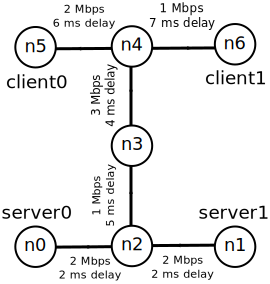
\includegraphics[width=2.5in]{topology}
\caption{The network testbed topology}
\label{fig_topology}
\end{figure}

In the server evaluation we have seen that the node adjacent to the server 
receives the CacheCast packets in the correct format. Now we need to test that 
the CMU and the CSU handles the packets correctly. Our most simple approach to 
this is to only enable server0 and client0. Then we only have a single list of 
nodes in which the start node is the server and the end node is the client. To 
prove that the CacheCast packet handling is correct in this simple scenario we 
connect, for each node, to the four trace sources explained above, and prints 
the time and the packet size. An example of this output for node 3 is 
presented in listing \ref{list_test1}. Each line in the following listings 
correspond to one packet being processed. We add 3 clients to the client0 node and use a packet with a 
size of 1000 bytes. The UDP header is 8 bytes, the IP header is 20 bytes, the 
CacheCast header is 10 bytes and the point-to-point header is 2 bytes, which 
adds up to 40 bytes of total header size.

\begin{lstlisting}[language=C, showstringspaces=false, 
basicstyle=\ttfamily\footnotesize, frame=tb, caption=Intercepted packets, 
label=list_test1]
Time (sec)  Packet size
1.01948     1040    \
1.0198      40       }  CcPreRecv (before CSU)
1.02012     40      /

1.01948     1030    \
1.0198      1030     }  CcPostRecv (after CSU)
1.02012     1030    /

1.01948     1030    \
1.02225     1030     }  CcPreSend (before CMU)
1.02236     1030    /

1.01948     1040    \
1.02225     40       }  CcPostSend (after CMU)
1.02236     40      /
\end{lstlisting}

We see in listing \ref{list_test1} that just before the CSU handles the packets we have the packet 
train structure. When the packets are processed on the node the CacheCast header 
(which is 10 bytes long) is removed and the packets are handled as normal IP 
packets. Then we see that the familiar packet train structure is again formed by 
the CMU. We observed that the packets, at the end, were correctly received on the client 
side. This test proves that the CacheCast technique does work in simple 
scenarios like this. But the reality is not as simple as this, so lets add a bit 
more complexity to the picture.

Now we enable the second server and client. This introduces (at least) two more 
potential points where implementation errors might be revealed; node 2, where 
two server channels join into one channel, and node 4 where the joint channel is 
split. Since the CMU identifies the CacheCast packet based on both the IP 
address and the payload ID the introduction of another server should not lead to 
other errors. The two servers send packets with a different 
size in order to differentiate them. Server0 sends three packets to client0 
and two packets to client1, while server1 sends one packet to client0 and three 
packets to client1. A similar output as in the previous test can be seen in 
listing \ref{list_test2}. The output is from node 3.

\begin{lstlisting}[language=C, showstringspaces=false, 
basicstyle=\ttfamily\footnotesize, frame=tb, caption=Intercepted packets with 
two servers, label=list_test2]
Time (sec)  Size   Source    Dest
1.00576     930    10.1.2.1  10.1.5.2
1.01328     930    10.1.2.1  10.1.6.2
1.0136      930    10.1.2.1  10.1.6.2
1.01392     1030   10.1.1.1  10.1.5.2
1.02224     930    10.1.2.1  10.1.6.2
1.02256     1030   10.1.1.1  10.1.5.2
1.02288     1030   10.1.1.1  10.1.5.2
1.0232      1030   10.1.1.1  10.1.6.2
1.02352     1030   10.1.1.1  10.1.6.2

After CMU
1.00576     940    10.1.2.1  10.1.5.2
1.01328     40     10.1.2.1  10.1.6.2
1.0136      40     10.1.2.1  10.1.6.2
1.01392     1040   10.1.1.1  10.1.5.2
1.02224     40     10.1.2.1  10.1.6.2
1.02256     40     10.1.1.1  10.1.5.2
1.02288     40     10.1.1.1  10.1.5.2
1.0232      40     10.1.1.1  10.1.6.2
1.02352     40     10.1.1.1  10.1.6.2
\end{lstlisting}

From the output we see that the packets originating from the two servers are mixed 
together when sent onto the channel after node 3. This is what one might expect. 
We can see that at this node the correct packets are truncated and the test 
showed that all the nodes handled the packets in the correct way. The clients 
received the correct number of packets with the correct payload attached.

Next we change the transmission rate on the channel between node2 and node3 to 
10Kbps. We do this in order to test the invalidation of payloads IDs which have been present in 
the cache for more than one second. Then we get the output shown in listing 
\ref{list_test3}, which is the packets traversing the link between n3 and n4. 

\begin{lstlisting}[language=C, showstringspaces=false, 
basicstyle=\ttfamily\footnotesize, frame=tb, caption=Intercepted packets with 
slow link, label=list_test3]
Time (sec)  Size   Source    Dest
1.76276     940    10.1.2.1  10.1.5.2
1.79476     40     10.1.2.1  10.1.6.2
1.82676     40     10.1.2.1  10.1.6.2
2.65876     1040   10.1.1.1  10.1.5.2
3.41076     940    10.1.2.1  10.1.6.2
4.24276     1040   10.1.1.1  10.1.5.2
4.27476     40     10.1.1.1  10.1.5.2
4.30676     40     10.1.1.1  10.1.6.2
4.33876     40     10.1.1.1  10.1.6.2
\end{lstlisting}

In this output we can see that the fifth and sixth packet from the top is not truncated. 
This is because more than one second has passed since the payload ID was cached.

In all the preceding tests the table/cache size and slot size have been large 
enough to hold all the packets. Now we change the size of the table and cache to 
10 with a slot size of 100 bytes, and resets previously changes the transmission 
rate. Introducing these changes tests two things; the handling of multiple slots per payload and the 
cache replacement mechanism. For the issue of multiple slots we compare the 
indices in which the payload should be stored, with the actual payload sizes of 
the packets and observe that the correct slots are in fact used. For the second 
issue we create a new output like in the previous tests. What we observe is 
that, besides that time stamps, the output is equal to the one in listing 
\ref{list_test3}. This seems very reasonable since the cache and table with the 
current size has only room for one packet (by using the aforementioned packet 
sizes). So each time a packet with a different global id than the previous one 
enters the CMU it has to be cached.

We finish this evaluation with a test concerning packet loss. Packet loss in a router does 
not affect CacheCast since CacheCast packets are handled like normal IP packets 
within routers. Thus we do not need to test for this explicitly. The only place 
where packet loss affects the CacheCast technique on the link. And there we have two types of 
packets which might get lost; truncated packet and non-truncated packets. We 
deal with the truncated packets first. A truncated packet does not carry any 
payload, thus no CSU state should be changed when a truncated packet is received. 
Hence, if a truncated packet is lost on the channel, it should not affect the 
CSU. So we construct a simple logic to remove a truncated packet from a link and 
observe the consequences. Our observations shows what we expected. No harm is 
done to the CSU because of the packet loss. Next we change our logic to remove a 
non-truncated packet. What we observe now is that when a non-truncated packet is 
lost on the channel, the whole packet train following it is also lost. As 
discussed by Srebrny\cite{srebrny}, this is a consequence of the CacheCast 
technique. When the packet carrying payload is lost, an inconsistency between 
the CMU's table and the CSU's is introduced. Therefore we must discard the other
truncated packets with the same global id. Our tests show that our 
implementation handles, in the correct way, all packet loss which might affect the CacheCast 
technique.


\section{Conclusion\label{s6}}
The conclusion goes here.

what is made:
    demos in example dir

\subsection{Future work}
The current implementation of CacheCast in ns-3 contains the features explained 
throughout this paper. This last section explains some of the work that might be 
done to the CacheCast module in the future.

1) The implementation of CacheCast in Linux supports both the UDP and DCCP 
transport protocols. In ns-3 there is currently no implementation of the DCCP 
protocol. If DCCP support is added to ns-3 in the future, the CacheCast 
module could be adapted to support this transport protocol.

2) Our implementation uses the PointToPointNetDevice as a basis for the 
CacheCastNetDevice. The PointToPointNetDevice does not model an ethernet link, 
just a general point-to-point link. To further enhance the realism in the 
CacheCast module, the CacheCastNetDevice should support ethernet links. 
In version 3.13 of ns-3 (which we rely on) does not have support for switched 
ethernet, but this support is currently being implemented in ns-3. Hence, support for 
ethernet links may be easily added to the CacheCast modules in the future.

3) Lastly, there is one issue which is not handle by current implementations of 
CacheCast. This issue arises most probably only with cache sizes with room for 
only one packet. First a CacheCast packet is sent and cached on the CSU. Then no 
packets are sent for 1 second. Then a new packet train is sent with the same 
payload ID and index as the previous packet. Then the first packet in the packet train is 
lost on the link. Then when the rest of the packets are processed by the CSU, 
the wrong payload is added to the packets. This issue might be easily solved by 
storing a time stamp together with the payload ID in the CSU.


% \appendices
% \section{Proof of the First Zonklar Equation}
% Appendix one text goes here.
% 
% % you can choose not to have a title for an appendix
% % if you want by leaving the argument blank
% \section{}
% Appendix two text goes here.


\section*{Acknowledgment}
The authors would like to thank their always positive and helpful supervisor Piotr 
Srebrny for useful guidelines and input in time of need.

\bibliography{library}
\bibliographystyle{IEEEtran}

\section*{Contributions}

\begin{tabular}{|l||p{5.3cm}|}
\hline
Bekzhan & \textbf{Report:}\\
Kassymbekov & -~Network implementation (Lancaster version)\\
& -~Network support evaluation\\
& \textbf{Implementation:}\\
& -~CacheManagementUnit (Lancaster version)\\
& -~CacheStoreUnit (Lancaster version)\\
\hline
Dag~Henning & \textbf{Report:}\\
Liodden~S�rb� & -~The CacheCast system\\
& -~General implementation details\\
& \emph{Server support implementation:}\\
& -~Underlying packet handling mechanism\\
& \emph{Network support (Oslo version):}\\
& -~CMU\\
& -~CacheCast module evaluation\\
& -~Future work\\
& \textbf{Implementation:}\\
& -~CacheCastHeader\\
& -~CacheCastNetDevice\\
& -~CacheCastTag\\
& -~CacheManagementUnit (Oslo version)\\
& -~CacheCastServerUnit\\
& -~CacheCast helpers\\
& -~CacheCast examples\\
\hline
Kanat & \textbf{Report:}\\
Sarsekeyev & -~Network implementation (Lancaster version)\\
& -~Network support evaluation\\
& \textbf{Implementation:}\\
& -~CacheManagementUnit (Lancaster version)\\
& -~CacheStoreUnit (Lancaster version)\\
\hline
Rizwan & \textbf{Report:}\\
Ali~Ahmed & -~The ns-3 network simulator\\
& -~Application programming interface (API)\\
& \emph{Server support implementation:}\\
& -~Details of the API implementation\\
& \emph{Network support (Oslo version):}\\
& -~CSU\\
& -~Server support evaluation\\
& \textbf{Implementation:}\\
& -~CacheCast container\\
& -~Msend() function\\
& -~CacheStoreUnit (Oslo version)\\
\hline
\end{tabular}


%%---------------------------------------------------------------------------%%
\end{document}


% EXAMPLES

%\begin{figure}[!t]
%\centering
%\includegraphics[width=2.5in]{myfigure}
%\caption{Simulation Results}
%\label{fig_sim}
%\end{figure}

%\begin{table}[!t]
%% increase table row spacing, adjust to taste
%\renewcommand{\arraystretch}{1.3}
% if using array.sty, it might be a good idea to tweak the value of
% \extrarowheight as needed to properly center the text within the cells
%\caption{An Example of a Table}
%\label{table_example}
%\centering
%% Some packages, such as MDW tools, offer better commands for making tables
%% than the plain LaTeX2e tabular which is used here.
%\begin{tabular}{|c||c|}
%\hline
%One & Two\\
%\hline
%Three & Four\\
%\hline
%\end{tabular}
%\end{table}

